\usetikzlibrary{arrows}
\begin{figure}[h]
	\centering
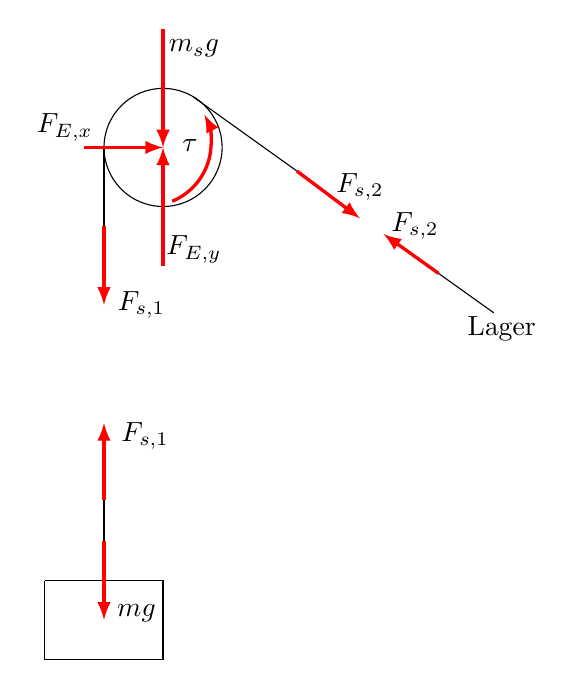
\begin{tikzpicture}
\draw (-3.5,-1) -- (-3.5,-2) -- (-2,-2) -- (-2,-1) -- (-3.5,-1);
\draw (-2.75,-1) -- (-2.75,0.5);
\draw [-latex][red,very thick](-2.75,0.0232) -- (-2.75,1.0);
\draw[-latex][red,very thick](-2.75,-0.5) -- (-2.75, -1.5);
\draw (-2.3377,-1.4121) node {\( mg\)} ;
\draw (-2.228,0.8364) node {\( F_{s,1}\)};
\draw (-1.62,5.145) -- (-0.3,4.2);
\draw  (-2,4.5) circle (0.75);
\draw (-2.75,4.5) -- (-2.75,3.5);
\draw [-latex][red,very thick](-2.75,3.5) -- (-2.75,2.5);
\draw [-latex][red,very thick] (-3,4.5) -- (-2,4.5);
\draw [latex-][red,very thick]  (-2,4.5) -- (-2,6);
\draw [latex-][red,very thick]  (-2,4.5) -- (-2,3);
\draw [-latex][red,very thick](-1.8834,3.8167) arc (-67.5126:26.8608:0.8);
\node at (-2.2741,2.505) {\(F_{s,1}\)};
\node at (-1.6074,3.205) {\( F_{E,y}\)};
\node at (-3.249,4.755) {\(F_{E,x}\)};
\node at (-1.6074,5.755) {\(m_sg\)};
\node at (-1.6574,4.5217) {\( \tau\)};
\draw [-latex][red,very thick] (-0.3,4.2) --(0.5,3.6);
\node at (0.5,4) {\( F_{s,2}\)};
\draw [latex-][red,very thick](0.8,3.4) -- (1.5,2.9);
\draw (1.5,2.9) -- (2.2,2.4);
\node at (1.2,3.5) {\(F_{s,2}\)};
\node at (2.3,2.2) {Lager};
\end{tikzpicture}
\end{figure}